\section{Implementation and Numerical Results}
\label{sec:84results}

\minitoc[3mm]{65mm}{6}

\parbox{1em}{}
\vspace{-3em}



\disableornamentsfornextheadingtrue
\subsection{Implementation}
\label{sec:841implementation}

\paragraph{Parameter values}

We used
a risk aversion factor of $\riskav \ceq 3.5$,
a patience factor of $\patience \ceq 0.97$,
a transaction cost rate of $\tac \ceq \SI{1}{\percent}$, and
a minimum consumption of $\normconsume_{\min} \ceq 0.001$.
The bond and stock return rates $\bondreturn_t$ and $\vstockreturn_t$
were taken from \cite{Cai10Stable};
the log-normally distributed stock return rates were generalized
from the three-stock case to five stocks via
$\ln \vstockreturn_t \sim \mathcal{N}(\*\mu, \mat{\Sigma})$, where
{%
  \setlength{\abovedisplayskip}{6pt}%
  \setlength{\belowdisplayskip}{6pt}%
  \begin{equation}
    \label{eq:financeStockReturnMeanCovariance}
    \*\mu
    \ceq
    \scalebox{0.92}{$
      \begin{pmatrix*}[l]
        0.0572\\
        0.0638\\
        0.07\\
        0.0764\\
        0.0828
      \end{pmatrix*}
    $},\quad
    \mat{\Sigma}
    \ceq 10^{-2}
    \scalebox{0.92}{$
      \begin{pmatrix*}[l]
        2.56&  0.576&   0.288&   0.176&  0.096\\
        0.576& 3.24&    0.90432& 1.0692& 1.296\\
        0.288& 0.90432& 4&       1.32&   1.68\\
        0.176& 1.0692&  1.32&    4.84&   2.112\\
        0.096& 1.296&   1.68&    2.112&  5.76
      \end{pmatrix*}
    $}.
  \end{equation}%
}%
The models were solved for $T = 6$ time steps;
this number suffices to show all relevant numerical effects and results,
while keeping the computational effort at a reasonable level.
As initial grids, we employed regular sparse grids
$\coarseregsgset{n}{d}{b}$ with $b = 1$
to decrease the number of grid points
(see \cref{sec:241coarseBoundary}).

\vspace*{0.25em}

\paragraph{Software}

The dynamic portfolio choice models were solved using a self-written
MATLAB framework.
The object-oriented framework was designed in such a way that
not only transaction costs problems,
but many other types of dynamic portfolio choice models can be handled.
For instance, the base class \texttt{LifecycleProblem} provides
an interface with abstract functions such as
\texttt{computeTerminalValueFunction} and
\texttt{computeStateTransition}.
The actual functionality implemented in the base class strongly resembles
the algorithms presented in \cref{sec:82algorithms}.
This is not only desirable from a modeling perspective,
but also facilitates future usage by other researchers.
For creating (i.e., hierarchizing) and evaluating sparse grid interpolants,
the sparse grid toolbox \sgpp was used \cite{Pflueger10Spatially}.%
\footnote{%
  \url{http://sgpp.sparsegrids.org/}%
}
The emerging optimization problems were solved using
sequential quadratic programming methods supplied by the
NAG Toolbox for MATLAB.%
\footnote{%
  \url{https://www.nag.com/}%
}
To avoid being stuck in local minima,
we repeated the optimization process for a varying number
of initial multi-start points (in the range of a few dozens).
All computation times were measured on a shared-memory computer
with 4x Intel Xeon E7-8880v3 (72 cores, 144 threads).



\subsection{Error Sources and Error Measure}
\label{sec:842errorSources}

\vspace*{0.25em}

\paragraph{Error sources}

In this application, there are the following error sources:

\begin{enumerate}[
  label=E\arabic*.,
  ref=E\arabic*,
  leftmargin=2.7em,
]
  \item
  \label{item:financeErrorInterpolationValue}
  Interpolation of the value function
  (i.e., $\normcetvalueintp_{t+1} \not= \normcetvaluefcn_{t+1}$)
  
  \item
  \label{item:financeErrorInterpolationPolicy}
  Interpolation of the policy functions
  (i.e., $\optnormpolicyintp_t \not= \optnormpolicyfcn_t$)
  
  \item
  \label{item:financeErrorExtrapolation}
  Extrapolation
  (i.e., $
  \normcetvalueintp_{t+1}(\state_{t+1})
  \not= \normcetvaluefcn_{t+1}(\state_{t+1})
  $)
  
  \item
  \label{item:financeErrorCropping}
  State space cropping
  (i.e., Euler errors do not vanish for exact solution)
  
  \item
  \label{item:financeErrorOptimization}
  Optimization
  (i.e., the minimum found by the optimizer is inaccurate or not global)
  
  \item
  \label{item:financeErrorQuadrature}
  Quadrature
  ($
    \expectation[t]{\cdots}
    \not= \sum_{j=1}^{m_{\quadweight}} \quadweight_t^{(j)}
    \cdot [\cdots](\stochastic_t^{(j)})
  $)
  
  \item
  \label{item:financeErrorRounding}
  Floating-point rounding errors
  (i.e., arithmetical operations are inaccurate)
\end{enumerate}
Due to the dynamic programming scheme,
the combination of all errors accumulates over $t$.
For instance, if the optimization does not find the global optimum
exactly or it only finds a local one for $t + 1$,
the error propagates from the interpolant $\normcetvalueintp_{t+1}$
on the right-hand side of the Bellman equation
\eqref{eq:normalizedTCPBellmanEquation} to $\normcetvalueintp_t$
on the left-hand side, and so on.
If the system does not damp these errors,
the error steadily becomes larger backwards in time $t$.

\paragraph{Error measure}

We use the weighted Euler equation error
$\weightedeulererror_t(\normstate_t)$
to assess the quality of the resulting policies
($\Ltwo$ norm or pointwise).
As the errors generally grow backwards in time,
it suffices to consider $t = 0$.
However, since Euler equation errors can only be evaluated at points in
the simplex
$
  \Omega_\mathrm{simplex}
  \ceq \{\normstate_t \in \clint{\*0, \*1} \mid \sumfcn(\normstate_t) \le 1\}
$, the $\Ltwo$ norm would
quickly converge to zero with growing dimensionality, even if the mean error
stayed constant.
Therefore, we normalize the $\Ltwo$ norm:
\begin{equation}
  \weightedeulererrorLtwo_t
  \ceq \sqrt{d!} \cdot \normLtwo{\weightedeulererror_t}
  = \sqrt{
    \frac{1}{\vol{\Omega_\mathrm{simplex}}}
    \int_{\mathrlap{\Omega_\mathrm{simplex}}\hphantom{\Omega}}
    \weightedeulererror_t(\normstate_t)^2 \diff{}\normstate_t
  },
\end{equation}
where the expression under the root sign is approximated
via Monte Carlo quadrature as the mean of samples
of $\weightedeulererror_t(\normstate_t)^2$.



\subsection{Numerical Results}
\label{sec:843results}

\paragraph{Full grid solution}

We show in \cref{fig:financeSolution2DReference}
a full grid solution for the case of $d = 2$ stocks,
i.e., $\{\state_t^{(k)} \mid k = 1, \dotsc, \ngp_t\} = \fgset{n,d}$
for some fixed level $n \in \nat$
(here, $n = 7$ and $\ngp_t = (2^7 + 1)^2 = \num{16641}$) and
for all $t = 0, \dotsc, T$.
Obviously, this is only computationally feasible
for low dimensionalities $d$ due to the curse of dimensionality.
The two-dimensional solution of level $n = 7$
took over nine hours to compute.
The solution of the next level is estimated to already take one week.
Hence, full grid solutions can only be computed up to $d = 3$
due to excessive computation time for $d \ge 4$.
This underlines the need for sophisticated
discretization techniques such as sparse grids.

\begin{figure}
  \makebox[49mm][r]{%
    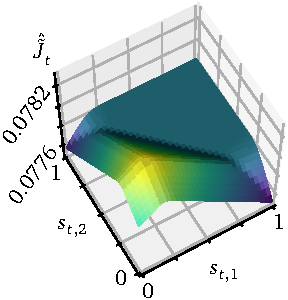
\includegraphics{financeSolution2D_1}%
  }%
  \hfill%
  \makebox[49mm][r]{%
    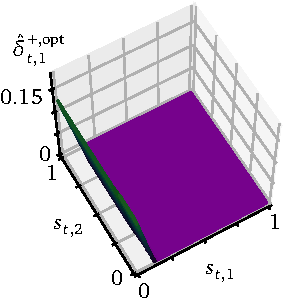
\includegraphics{financeSolution2D_2}%
  }%
  \hfill%
  \makebox[49mm][r]{%
    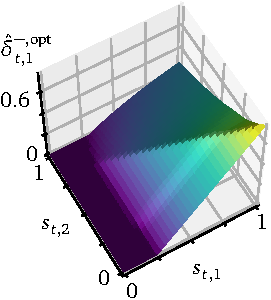
\includegraphics{financeSolution2D_4}%
  }%
  \\[0mm]%
  \makebox[49mm][r]{%
    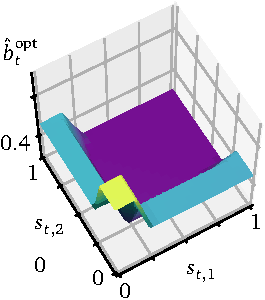
\includegraphics{financeSolution2D_6}%
  }%
  \hfill%
  \makebox[49mm][r]{%
    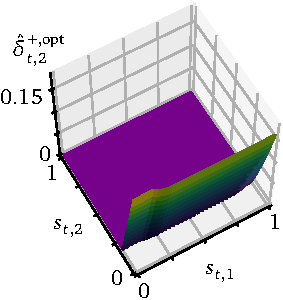
\includegraphics{financeSolution2D_3}%
  }%
  \hfill%
  \makebox[49mm][r]{%
    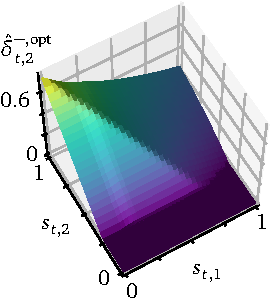
\includegraphics{financeSolution2D_5}%
  }%
  \caption[Reference solution for the two-dimensional TCP]{%
    Full grid solution for the transaction costs problem
    with $d = 2$ stocks.
    Shown are the value function $\normcetvaluefcn_t$ \emph{(top left)} and the
    optimal policy $\optnormpolicyfcn_t$ for $t = 0$.%
  }%
  \label{fig:financeSolution2DReference}%
\end{figure}

\paragraph{Convergence of the weighted Euler equation error}

\Cref{fig:financeEulerError} shows the convergence of the
$\Ltwo$ norm $\weightedeulererrorLtwo_0$ of the
weighted Euler equation error for $t = 0$ for regular sparse grids
and spatially adaptive sparse grids
for the cases of $d = 1, \dotsc, 4$ stocks.
\begin{figure}
  
\includegraphics{financeEulerError_5}%
  \\[2mm]%
  \subcaptionbox{%
    $d = 1$%
  }[37mm]{%
    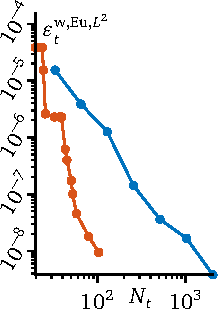
\includegraphics{financeEulerError_1}%
  }%
  \hfill%
  \subcaptionbox{%
    $d = 2$%
  }[37mm]{%
    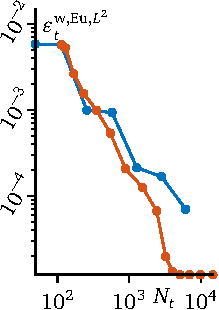
\includegraphics{financeEulerError_2}%
  }%
  \hfill%
  \subcaptionbox{%
    $d = 3$%
  }[37mm]{%
    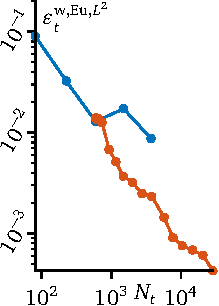
\includegraphics{financeEulerError_3}%
  }%
  \hfill%
  \subcaptionbox{%
    $d = 4$%
  }[37mm]{%
    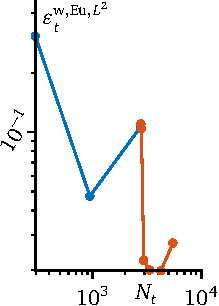
\includegraphics{financeEulerError_4}%
  }%
  \caption[Convergence of the weighted Euler equation error]{%
    Convergence of the $\Ltwo$ norm $\weightedeulererrorLtwo_t$
    of the weighted Euler equation error for $t = 0$ for
    regular sparse grids \emph{\textcolor{C0}{(blue)}} and
    spatially adaptive sparse grids \emph{\textcolor{C1}{(red)}.}
    The number $\ngp_t$ is the average number
    $\frac{1}{m_{\policy}} \sum_{j=1}^{m_{\policy}} \ngp_{t,j}$
    of grid points over all policy grids for $t = 0$,
    where $\ngp_{t,j}$ is the number of grid points
    of the $j$-th policy entry.%
  }%
  \label{fig:financeEulerError}%
\end{figure}%
For this and the following plots,
the value function grid is left unchanged
(usually a slightly refined regular sparse grid),
while the average number $\ngp_t$ of policy grid points increases
with decreasing refinement threshold $\refinetol_t$.
This is because the value function grid does not seem to have a great influence
on the convergence of the Euler equation errors.
Compared to regular grids, the spatial adaptivity decreases the error by
two orders of magnitude in one dimension.
The gain is smaller for higher dimensionalities $d$,
but spatially adaptive grids still outperform regular grids.
For $d = 2$, we observe that the error saturates
at $\ngp_t \approx \num{4000}$ points just above $10^{-5}$.
This is most likely due to the parts
\ref{item:financeErrorExtrapolation} to
\ref{item:financeErrorRounding} of the error that are not influenced
by sparse grid interpolation.
In addition, convergence significantly decelerates starting with $d = 4$.
For $d = 4$, spatially adaptive sparse grids
are able to achieve a weighted Euler equation error of
$\weightedeulererrorLtwo_t \approx \num{2.0e-2}$ for $t = 0$
(with an average number $\ngp_0 = \num{4252}$ of policy grid points).
For $d = 5$, we are still able to achieve a small error of
$\weightedeulererrorLtwo_t \approx \num{1.9e-2}$ for $t = 0$
with spatially adaptive sparse grids with
an average number $\ngp_0 = \num{12572}$ of policy grid points.
While we cannot detect any convergence for this dimensionality yet,
this is still a major result as such high-dimensional models
could not be solved up to now with conventional methods.

\paragraph{Optimal policies in 2D and 5D}

\Cref{fig:financeSolution2DSparseGrid,fig:financeSolution5DSparseGrid}
each display
\begin{figure}
  \subcaptionbox{%
    $\normcetvalueintp[1]_t$%
  }[48mm]{%
    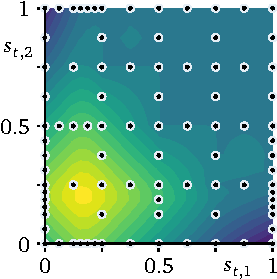
\includegraphics{financeSolution2D_7}%
  }%
  \hfill%
  \subcaptionbox{%
    $\normbuy[\opt,\sparse,1]_{t,1}$%
  }[48mm]{%
    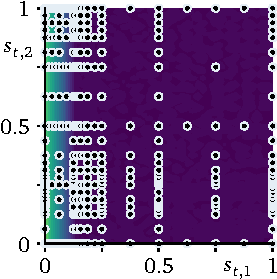
\includegraphics{financeSolution2D_8}%
  }%
  \hfill%
  \subcaptionbox{%
    $\normsell[\opt,\sparse,1]_{t,1}$%
  }[48mm]{%
    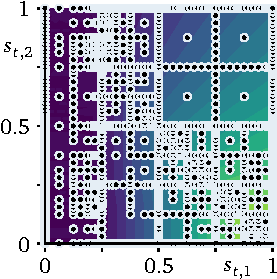
\includegraphics{financeSolution2D_10}%
  }%
  \\[2mm]%
  \subcaptionbox{%
    $\normbond_t^{\opt,\sparse,1}$%
  }[48mm]{%
    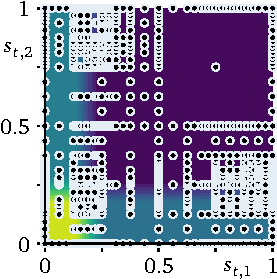
\includegraphics{financeSolution2D_12}%
  }%
  \hfill%
  \subcaptionbox{%
    $\normbuy[\opt,\sparse,1]_{t,2}$%
  }[48mm]{%
    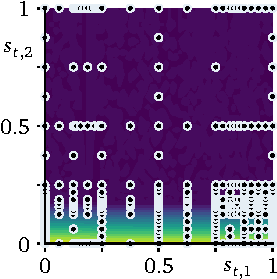
\includegraphics{financeSolution2D_9}%
  }%
  \hfill%
  \subcaptionbox{%
    $\normsell[\opt,\sparse,1]_{t,2}$%
  }[48mm]{%
    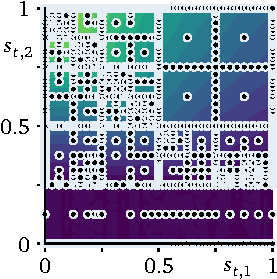
\includegraphics{financeSolution2D_11}%
  }%
  \caption[Sparse grid solution for the two-dimensional TCP]{%
    Spatially adaptive sparse grid solution for the transaction costs problem
    \vspace{-0.15em}%
    with $d = 2$ stocks.
    \vspace{-0.15em}%
    Shown are the value function $\normcetvalueintp_t$ \emph{(top left)} and the
    optimal policy $\optnormpolicyintp_t$ for the initial time step $t = 0$,
    together with the corresponding grid points \emph{(dots).}
    The color coding is the same as in
    \cref{fig:financeSolution2DReference}.%
  }%
  \label{fig:financeSolution2DSparseGrid}%
\end{figure}%
\begin{figure}
  \makebox[37mm][c]{%
    \hspace*{3.8mm}%
    \raisebox{-\height}{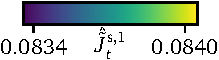
\includegraphics{financeSolution5D_13}}%
  }%
  \hfill%
  \makebox[37mm][c]{%
    \hspace*{3.8mm}%
    \raisebox{-\height}{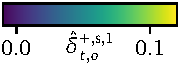
\includegraphics{financeSolution5D_14}}%
  }%
  \hfill%
  \makebox[37mm][c]{%
    \hspace*{4.4mm}%
    \raisebox{-\height}{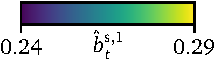
\includegraphics{financeSolution5D_16}}%
  }%
  \hfill%
  \makebox[37mm][c]{%
    \hspace*{2.4mm}%
    \raisebox{-\height}{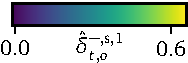
\includegraphics{financeSolution5D_15}}%
  }%
  \\[1mm]%
  \makebox[37mm][c]{%
    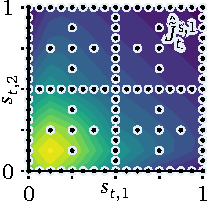
\includegraphics{financeSolution5D_1}%
  }%
  \hfill%
  \makebox[37mm][c]{%
    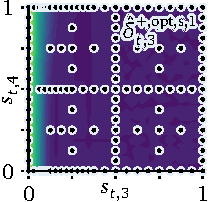
\includegraphics{financeSolution5D_4}%
  }%
  \hfill%
  \makebox[37mm][c]{%
    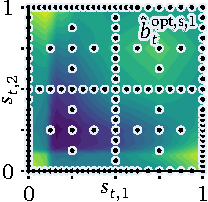
\includegraphics{financeSolution5D_12}%
  }%
  \hfill%
  \makebox[37mm][c]{%
    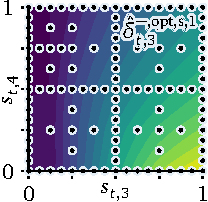
\includegraphics{financeSolution5D_9}%
  }%
  \\[1mm]%
  \makebox[37mm][c]{%
    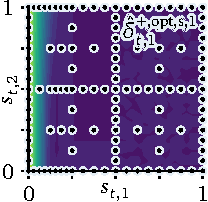
\includegraphics{financeSolution5D_2}%
  }%
  \hfill%
  \makebox[37mm][c]{%
    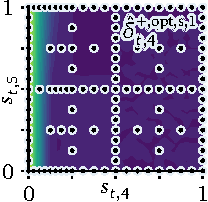
\includegraphics{financeSolution5D_5}%
  }%
  \hfill%
  \makebox[37mm][c]{%
    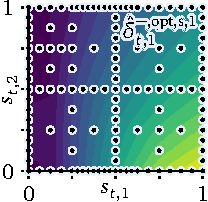
\includegraphics{financeSolution5D_7}%
  }%
  \hfill%
  \makebox[37mm][c]{%
    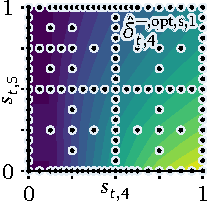
\includegraphics{financeSolution5D_10}%
  }%
  \\[1mm]%
  \makebox[37mm][c]{%
    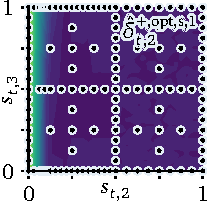
\includegraphics{financeSolution5D_3}%
  }%
  \hfill%
  \makebox[37mm][c]{%
    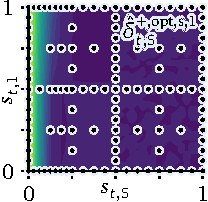
\includegraphics{financeSolution5D_6}%
  }%
  \hfill%
  \makebox[37mm][c]{%
    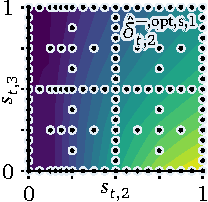
\includegraphics{financeSolution5D_8}%
  }%
  \hfill%
  \makebox[37mm][c]{%
    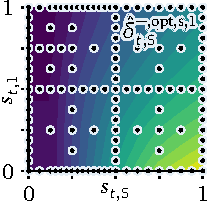
\includegraphics{financeSolution5D_11}%
  }%
  \caption[Sparse grid solution for the five-dimensional TCP]{%
    Spatially adaptive sparse grid solution for the transaction costs problem
    \vspace{-0.15em}%
    with $d = 5$ stocks.
    \vspace{-0.15em}%
    Shown are slice plots of
    the value function $\normcetvalueintp_t$ \emph{(top left)} and
    the optimal policy $\optnormpolicyintp_t$
    for the initial time step $t = 0$,
    where for each function, a pair $(o_1, o_2)$
    of dimensions to be plotted was chosen,
    and the stock fractions $\stock_{t,o}$ of the other dimensions $o$
    are set to $0.1$.
    In addition, the corresponding grid points \emph{(dots)}
    are shown as the projection onto the
    $\stock_{t,o_1}$-$\stock_{t,o_2}$ plane.%
  }%
  \label{fig:financeSolution5DSparseGrid}%
\end{figure}%
the value function and the optimal policies corresponding to
sparse grid solutions for
$d = 2$ stocks with $\ngp_0 = \num{879}$ policy grid points or
$d = 5$ stocks with $\ngp_0 = \num{12572}$ policy grid points.
Obviously, most grid points are placed along the various kinks in the
policies.
Interestingly, experiments show that the surplus-based refinement
criterion does not place more grid points along the perfectly diagonal kink
caused by the cropping of the state space
(i.e., along $\sumfcn(\vstock_t) = 1$).
It is possible to circumvent this issue by either
transforming the domain (e.g., rotations as in \cite{Bohn18Optimally}) or
directly incorporating the distance to the diagonal into the
refinement criterion for the value function.
However, we refrain from doing so here as this does not seem to
drastically improve results.
Again, this might be due to the domination of the overall error by
the parts \ref{item:financeErrorExtrapolation} to
\ref{item:financeErrorRounding} that are not related to interpolation.

\paragraph{Pointwise error}

Pointwise plots of the weighted Euler equation error
as in \cref{fig:financePointwiseError} for two stocks
reveal that there are two types of regions where the error is large:
The first type of region
is the neighborhood of the aforementioned diagonal boundary
$\sumfcn(\vstock_t) = 1$ of the uncropped region,
where the cropping distorts the error despite the weights.
The second type of region
are kinks of the optimal policy functions,
which is most visible for coarse grids
(e.g., \cref{fig:financePointwiseError_1}).
When increasing the number of grid points
(e.g., \cref{fig:financePointwiseError_1,fig:financePointwiseError_2}),
the error decreases quickly in the whole domain.

\begin{figure}
  \subcaptionbox{%
    $\ngp_t = 129$ (\num{5.3e-3})%
    \label{fig:financePointwiseError_1}%
  }[44mm]{%
    \clap{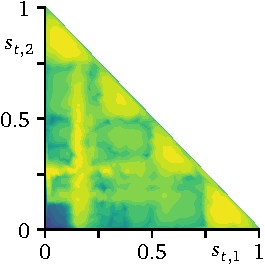
\includegraphics{financePointwiseError_1}}%
  }%
  \subcaptionbox{%
    $\ngp_t = 889$ (\num{2.1e-4})%
    \label{fig:financePointwiseError_2}%
  }[44mm]{%
    \clap{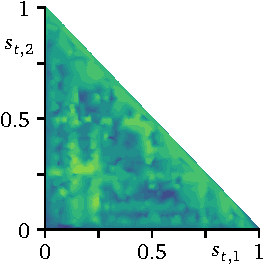
\includegraphics{financePointwiseError_2}}%
  }%
  \subcaptionbox{%
    $\ngp_t = 5159$ (\num{1.2e-5})%
    \label{fig:financePointwiseError_3}%
  }[44mm]{%
    \clap{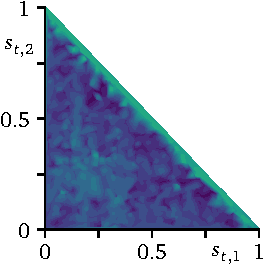
\includegraphics{financePointwiseError_3}}%
  }%
  \hfill%
  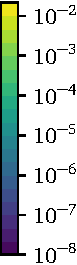
\includegraphics{financePointwiseError_4}%
  \caption[Pointwise weighted Euler equation error for different grids]{%
    Pointwise weighted Euler equation error $\weightedeulererror_t(\vstock_t)$
    ($t = 0$) for the two-dimensional transaction costs problem and
    different spatially adaptive sparse grids.
    The $\Ltwo$ error $\weightedeulererrorLtwo_t$ is given in
    parentheses.%
  }%
  \label{fig:financePointwiseError}%
\end{figure}

\paragraph{Monte Carlo simulation}

As explained in \cref{sec:828postProecessing},
we perform a multi-agent Monte Carlo simulation
and plot the resulting mean state and policy in \cref{fig:financeSimulation}
for $d = 3$, $4$, and $5$ stocks.
\begin{figure}
  
\includegraphics{financeSimulation_5}%
  \\[2mm]%
  \subcaptionbox{%
    $d = 3$ ($\ngp_0 = \num{28739}$)%
    \label{fig:financeSimulation_1}%
  }[48mm]{%
    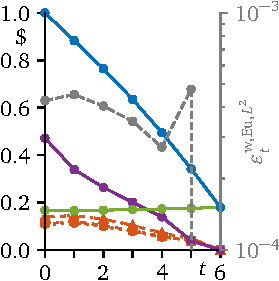
\includegraphics{financeSimulation_1}%
  }%
  \hfill%
  \subcaptionbox{%
    $d = 4$ ($\ngp_0 = \num{3343}$)%
    \label{fig:financeSimulation_2}%
  }[48mm]{%
    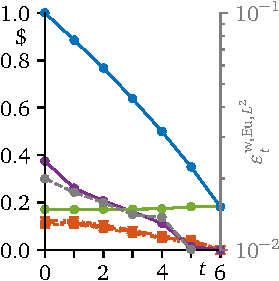
\includegraphics{financeSimulation_2}%
  }%
  \hfill%
  \subcaptionbox{%
    $d = 5$ ($\ngp_0 = \num{12572}$)%
    \label{fig:financeSimulation_3}%
  }[48mm]{%
    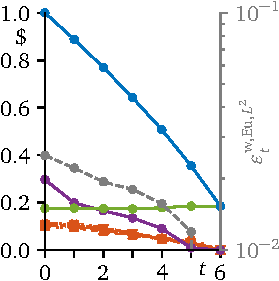
\includegraphics{financeSimulation_3}%
  }%
    \caption[Monte Carlo simulation of the TCP]{%
      Mean values of
      wealth $\wealth_t$
      \emph{\textcolor{C0}{(blue)},}
      unnormalized optimal bonds $\bond_t$
      \emph{\textcolor{C3}{(purple)},}
      unnormalized optimal consumption $\consume_t$
      \emph{\textcolor{C4}{(green)},} and
      unnormalized stock holdings
      $
        \acute{\vstock}_t
        \ceq (\vstock_t + \vnormbuy_t - \vnormsell_t) \wealth_t
      $
      after buying and selling
      \emph{\textcolor{C1}{(red)}}
      \vspace{0.1em}%
      in a Monte Carlo simulation of \num{10000} individuals,
      \vspace{-0.1em}%
      where we assume that $\wealth_0 = \$1$ for all individuals.
      In addition, the plots show the evolution of the
      $\Ltwo$ error $\weightedeulererrorLtwo_t$ over time $t$
      \emph{\textcolor{C8}{(gray, right axes)}.}%
    }%
    \label{fig:financeSimulation}%
\end{figure}%
In addition, this figure contains the evolution of the
weighted Euler equation error $\weightedeulererrorLtwo_t$ over time.
We perform a two-part assessment of the simulated results.
First, consumption should ideally be constant over time
from a finance perspective.
We measure this by calculating the coefficients of variation
(ratio of the standard deviation of the $c_t$ values to their mean),
which is \SI{2.76}{\percent}, \SI{2.68}{\percent}, and \SI{2.58}{\percent}
for $d = 3$, $4$, and $5$, respectively.
This indicates that the variation of the consumption over time
is indeed small.
Second, we consider the so-called \term{Sharpe ratios}
\cite{Sharpe66Mutual}.
The ratios are stock fractions $\vstock$ that are determined
such that the excess stock return (compared to risk-free investment)
per unit of risk is maximized:%
\footnote{%
  The Sharpe ratios per se are derived for non-skewed
  stock return rate distributions.
  Our stock return rates are log-normally distributed and thus skewed,
  but the deviation should be small after six time steps.
  However, there are variants that
  take skewed distributions into account \cite{Mueller15Ansaetze}.%
}
{%
  \setlength{\abovedisplayskip}{9pt}%
  \setlength{\belowdisplayskip}{9pt}%
  \begin{equation}
    \vecargmax_{\vstock \in \clint{0, 1}^d}
    \frac{
      \tr{\*\mu_{\range{1}{d}}} \vstock - \bondreturn
    }{
      \sqrt{\tr{\vstock} \mat{\Sigma}_{\range{1}{d},\range{1}{d}} \vstock}
    },
  \end{equation}%
}%
where $\*\mu_{\range{1}{d}}$ and
$\mat{\Sigma}_{\range{1}{d},\range{1}{d}}$
are the first $d$ entries of $\*\mu$ and
the principal minor of order $d$ of $\mat{\Sigma}$ as given in
\cref{eq:financeStockReturnMeanCovariance}.
We compare these theoretical Sharpe ratios (left)
with the simulated stock fractions
$\acute{\stock}_{t,o}/\sumfcn(\acute{\vstock}_t)$ for $t = 0$ (right):
\begin{subequations}
  \setlength{\jot}{3pt}%
  \begin{align}
    d = 3\colon\,&
    (0.314, 0.302, 0.384\rlap{),}\hphantom{, 0.999, 0.999}\quad
    (0.300, 0.317, 0.383),\\
    d = 4\colon\,&
    (0.275, 0.185, 0.250, 0.289\rlap{),}\hphantom{, 0.999}\quad
    (0.239, 0.238, 0.253, 0.270),\\
    d = 5\colon\,&
    (0.275, 0.122, 0.176, 0.203, 0.223\rlap{),}\quad
    (0.199, 0.188, 0.197, 0.205, 0.212).
  \end{align}
\end{subequations}
The simulated stock fractions
match the predicted Sharpe ratios well for $d = 3$,
while the deviation for $d \ge 4$ is larger.
However, as the simulated stock fractions do not change much over time,
we may suspect that the skewness of the distribution of the stock return rates
limits the applicability of the Sharpe ratios to these cases.

\paragraph{Complexity and computation time}

A complexity analysis reveals that the difficulty of solving
transaction cost problems quickly grows with the dimensionality $d$:
As shown in \cref{fig:structureSolveValueFunction},
the number of necessary arithmetic operations grows like
{%
  \setlength{\abovedisplayskip}{6pt}%
  \setlength{\belowdisplayskip}{6pt}%
  \begin{equation}
    \landauTheta{
      T
      \cdot \ngp_t
      \cdot \text{\#optimizer iterations}
      \cdot
      \underbrace{
        m_{\zeta}
        \cdot
        \overbrace{
          m_{\policy}
          \cdot
          \ngp_{t+1}
          \cdot m_{\state}
          \cdot p
        }^{\mathclap{\text{one evaluation of interpolant}}}
      }_{\mathclap{\text{one evaluation of objective gradient}}}\,
    },
  \end{equation}%
}%
where $m_{\state}, m_{\policy} \in \landauTheta{d}$ and
$m_{\zeta}, \ngp_t, \ngp_{t+1} \in \landauTheta{2^n n^{d-1}}$
if regular sparse grids of level $n$
without boundary points are used for state and stochastic grids
(due to $m_{\stochastic} = d$).
In addition,
the number of optimizer iterations is likely superlinear in $d$,
as this depends on the dimensionality $m_{\policy}$ of the search space
as well as on the number of multi-start points
(which also grows with $m_{\policy}$).
This means that the complexity is at least cubic in $d$,
quadratic in the average number $\ngp$ of employed state grid points, and
linear in the number $m_{\zeta}$ of quadrature points.
\Cref{fig:financeRuntime} confirms these observations with
experimental data.
\begin{figure}
  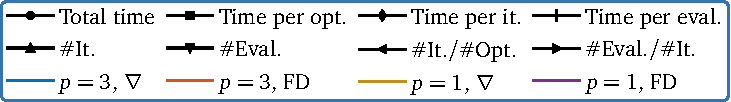
\includegraphics{financeRuntime_7}%
  \\[1mm]%
  \subcaptionbox{%
    $d = 1$%
  }[49.5mm]{%
    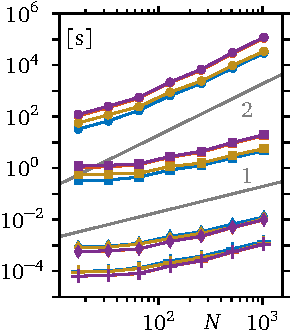
\includegraphics{financeRuntime_1}%
    \vspace*{0.3mm}\newline\hspace*{1.0mm}%
    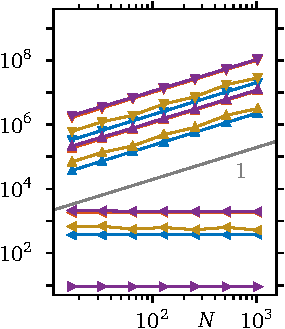
\includegraphics{financeRuntime_2}%
  }%
  \hfill%
  \subcaptionbox{%
    $d = 2$%
  }[49.5mm]{%
    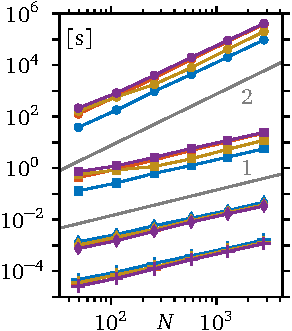
\includegraphics{financeRuntime_3}%
    \vspace*{0.3mm}\newline\hspace*{1.0mm}%
    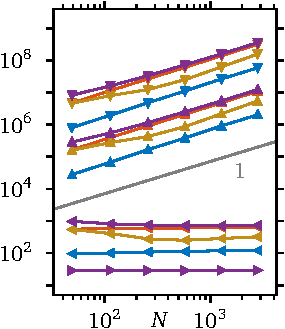
\includegraphics{financeRuntime_4}%
  }%
  \hfill%
  \subcaptionbox{%
    $d = 3$%
  }[49.5mm]{%
    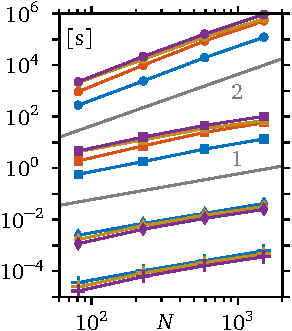
\includegraphics{financeRuntime_5}%
    \vspace*{0.3mm}\newline\hspace*{1.0mm}%
    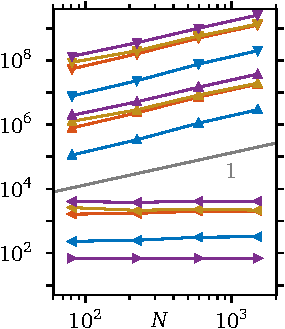
\includegraphics{financeRuntime_6}%
  }%
  \caption[Computation times and numbers of iterations for the TCP]{%
    Computation times \emph{(top)} and
    numbers of iterations and evaluations of the interpolant \emph{(bottom)}
    for the transaction costs problem on static regular sparse grids
    (i.e., without refinement).
    ``Total time'' is the serial time required to solve all
    emerging optimization problems.
    ``Time per opt.''\ is this time divided by the number
    $\mathrm{\#Opt.} = T\ngp$ of optimization problems.
    ``Time per it.''\ is the time divided by the number
    \#It.\ of optimization iterations,
    each of which is assumed to correspond to
    exactly one combined evaluation of objective function and gradient
    (the latter only if gradients are used).
    ``Time per eval.''\ is the time divided by
    the number \#Eval.\ of evaluations of
    the sparse grid interpolant and its gradient.
    The colors correspond to B-spline degrees $p = 3$ or $p = 1$ and
    to using gradients (``$\nabla$'') or finite differences (``FD'').%
  }%
  \label{fig:financeRuntime}%
\end{figure}%
For fixed $d$, the total time required by the optimization process
grows quadratically with the number $\ngp$ of grid points.
The time for one solution of the Bellman equation,
the time for one optimizer iteration, and
the time for one evaluation of the interpolant are all linear in $\ngp$,
as the number of optimizer iterations
is constant for fixed $d$.
If $d$ increases,
then the number of interpolant evaluations per optimizer iteration
(i.e., the number of quadrature points) increases as well.
Surprisingly, the number of optimizer iterations per grid point
and the time per evaluation are not monotonously increasing.
The latter observation might be due to vectorization effects.

\paragraph{Comparison to piecewise linear functions}

Hierarchical B-splines introduce two major benefits to
the solution of dynamic portfolio choice models.
The first benefit are the smooth objective functions:
When repeating the computations with piecewise linear functions (i.e., $p = 1$),
one obtains almost the same weighted Euler equation errors as in the cubic case
(except for the case of $d = 1$, where the error is one order of
magnitude greater than in the cubic case).
However, as we see in \cref{fig:financeRuntime},
the total computation time is several times larger
(e.g., more than five times for $d = 3$) for piecewise linear functions,
although evaluations are cheaper than for B-splines.
The main reason is that the number of required optimizer iterations
is for $p = 1$ almost seven times as high as in the cubic case,
since the optimizer has to deal with kinks in the objective function.
Experiments show that beginning with $d = 4$,
the total optimization time required to solve the transaction costs problem
is one whole order of magnitude shorter for cubic B-splines
than for piecewise linear functions.

\paragraph{Comparing exact gradients to finite differences}

The second benefit is the availability of exact gradients:
\Cref{fig:financeRuntime} also contains computation times of the
solution process
if we artificially do not use exact gradients of the objective functions,
but rather approximate them with finite differences.
For each evaluation of the objective gradient,
at least $m_{\policy}$ additional evaluations of the objective function
have to performed to compute the finite differences
($2m_{\policy}$ if central differences are used).
Consequently, while the resulting weighted Euler equation errors are
similar, the total optimization time roughly increases by a
factor of up to five if we do not use exact gradients.
